%%%%%%%%%%%%%%%%%%%%%%%%%%%%%%%%%%%%%%%%%%%%%%%%%%%%%%%%%%%%%%%%%%%%%%%%%%%%%%%%%%%%%%%%%%%%%%
% Template Beamer Sugestivo para Projetos no Senac
% by ezefranca.com
% Based on MIT Beamer Template
% As cores laranja e azul seguem o padrao proposto no manual de uso da identidade visual senac
%%%%%%%%%%%%%%%%%%%%%%%%%%%%%%%%%%%%%%%%%%%%%%%%%%%%%%%%%%%%%%%%%%%%%%%%%%%%%%%%%%%%%%%%%%%%%% 

%\documentclass{beamer} %voce pode usar este modelo tambem
\documentclass[handout,t]{beamer}
\usepackage{graphicx,url}
\usepackage{subcaption,rotating,natbib}
%\usepackage[english]{babel}   
\usepackage[utf8]{inputenc}
%\batchmode
% \usepackage{pgfpages}
% \pgfpagesuselayout{4 on 1}[letterpaper,landscape,border shrink=5mm]
\usepackage{amsmath,amssymb,enumerate,epsfig,bbm,calc,color,ifthen,capt-of}
\usetheme[compress]{Berlin}
%\usetheme[compress]{Singapore}
\usepackage{booktabs} % Allows the use of \toprule, \midrule and \bottomrule in tables
\usepackage{appendixnumberbeamer}
\DeclareUnicodeCharacter{394}{$\Delta$}

\newcommand{\specialcell}[2][c]{%
	\begin{tabular}[#1]{@{}c@{}}#2\end{tabular}}

\newcommand\partt[2][]{\ensuremath{\frac{\partial#1}{\partial#2}}} %the [2] indicates there will be 2 elements. This command defines a partial derivative where 2 arguments are numerator and denominator.
\usepackage[none]{hyphenat}
\usepackage{tikz}
\usepackage{verbatim}
\usetikzlibrary{arrows,calc, patterns, positioning, shapes.geometric, decorations.pathreplacing,decorations.markings}
\usepackage{graphicx}
\usepackage{rotating}
\usepackage{textcomp}
\hypersetup{
     colorlinks=true,
     linkcolor=white,
     filecolor=blue,      
     urlcolor=blue,
     citecolor=black,
 }
%\usepackage[backend=biber]{biblatex}
%\usepackage{biblatex}
%\usepackage[style=authoryear]{biblatex}
%\usepackage{natbib}

%\usepackage[natbib=true,style=authoryear,backend=bibtex,useprefix=true]{biblatex}
%\addbibresource{Bib.bib}

\setbeamertemplate{headline}
{%
	\begin{beamercolorbox}[colsep=1.5pt]{upper separation line head}
	\end{beamercolorbox}
	\begin{beamercolorbox}{section in head/foot}
		\vskip2pt\insertnavigation{\paperwidth}\vskip2pt
	\end{beamercolorbox}%
	\begin{beamercolorbox}[colsep=1.5pt]{lower separation line head}
	\end{beamercolorbox}
}

\setbeamertemplate{blocks}[rounded][shadow=true]
\setbeamertemplate{footline}[frame number]{}

%-------------------------Este código faz o menuzinho bacana na parte superior do slide------------
\AtBeginSection[]
{
  \begin{frame}<beamer>
    \frametitle{Outline}
    \tableofcontents[currentsection]
  \end{frame}
}
\beamerdefaultoverlayspecification{<+->}
% -----------------------------------------------------------------------------
% \begin{document}
% % -----------------------------------------------------------------------------

% %---Gerador de Sumário---------------------------------------------------------
% \frame{\titlepage}
% \section[]{}
% \begin{frame}{Outline}
%   \tableofcontents
% \end{frame}
% %---Fim do Sumário------------------------------------------------------------


% % Para cambiar los colores de los diferentes elementos en la presentación, descomente y edite las siguitenes líneas

% % Cambiar el color de las barras:
% \setbeamercolor{Feather}{fg=structColor!50,bg=barColor}

% % Cambiar el color de los elementos estructurales
% \setbeamercolor{structure}{fg=structColor}

% % Cambiar el color del título de las diapositivas
% \setbeamercolor{frametitle}{fg=titlesColor}

% % Cambiar el color del fondo de la diapositiva
% \setbeamercolor{normal text}{fg=black, bg=backColor!35}

%-------------------------------------------------------
% PAQUETES INCLUIDOS
%-------------------------------------------------------

\usepackage[utf8]{inputenc}
\usepackage{soulutf8}
\usepackage[spanish, es-tabla]{babel}
\usepackage{amsmath}
\usepackage{amsfonts}
\usepackage{amssymb}
\usepackage{helvet}
\usepackage{graphicx}
\usepackage{tikz}
\usetikzlibrary{
	calc, angles, quotes, positioning,
    babel, shapes, arrows, shadows
    }
\usepackage{tkz-fct}
\usepackage{circuitikz}
\usetikzlibrary{babel}
\usepackage{subcaption}
\usepackage{calc}
\usepackage{multirow, multicol}
\usepackage{xcolor}
\usepackage{xkeyval}
\usepackage{minted}
\RequirePackage{etex}

%-------------------------------------------------------
% DEFINICIÓN Y REDEFINICIÓN DE COLORES
%-------------------------------------------------------
\definecolor{structColor}{HTML}{201090} % 015793
\definecolor{barColor}{HTML}{202122} % 202122
\definecolor{backColor}{HTML}{8998B5} % 8998B5
\definecolor{titlesColor}{HTML}{008100} % FF6614
\definecolor{myBlue}{HTML}{027FDF}
\definecolor{myGray}{HTML}{181818}
\definecolor{myRed}{HTML}{AA3939}
\definecolor{myGreen}{HTML}{32AB77}
\definecolor{myOrange}{HTML}{FF6302}

%-------------------------------------------------------
% DEFINICIÓN Y REDEFINICIÓN DE COMANDOS
%-------------------------------------------------------

% color de los hyperenlaces
\newcommand{\chref}[2]{
  \href{#1}{{\usebeamercolor[bg]{Feather}#2}}
}
\newcommand{\bftt}[1]{\textbf{\texttt{#1}}}
\newcommand*\keystroke[1]{%
  \tikz[baseline=(key.base)]
    \node[%
      draw,
      fill=white,
      drop shadow={shadow xshift=0.25ex,shadow yshift=-0.25ex,fill=black,opacity=0.75},
      rectangle,
      rounded corners=2pt,
      inner sep=1pt,
      line width=0.5pt,
      font=\scriptsize\sffamily
    ](key) {#1\strut}
  ;
}
\newcommand{\keystrokebftt}[1]{\keystroke{\bftt{#1}}}
\newcommand{\comment}[1]{{\color[HTML]{008080}\textit{\textbf{\texttt{#1}}}}}
\newcommand{\cmd}[1]{{\color[HTML]{008000}\bftt{#1}}} % comandos
\newcommand{\bs}{\char`\\}
\newcommand{\cmdbs}[1]{\cmd{\bs#1}}
\newcommand{\lcb}{\char '173}
\newcommand{\rcb}{\char '175}
\newcommand{\cmdbegin}[1]{\cmdbs{begin\lcb}\bftt{#1}\cmd{\rcb}}
\newcommand{\cmdend}[1]{\cmdbs{end\lcb}\bftt{#1}\cmd{\rcb}}
\newcommand{\wllogo}{\textbf{Overleaf}}
\newenvironment{exampletwouptiny}
  {\VerbatimEnvironment
   \begin{VerbatimOut}{example.out}}
  {\end{VerbatimOut}
   \setlength{\parindent}{0pt}
   \fbox{\begin{tabular}{l|l}
   \begin{minipage}{0.62\linewidth}
     \inputminted[fontsize=\scriptsize,resetmargins]{latex}{example.out}
   \end{minipage} &
   \begin{minipage}{0.35\linewidth}
     \setlength{\parskip}{6pt plus 1pt minus 1pt}%
     \raggedright\scriptsize\input{example.out}
   \end{minipage}
   \end{tabular}}}
%-------------------------------------------------------
% INFORMACIÓN EN LA CABECERA DE PÁGINA
%-------------------------------------------------------

\title[\LaTeX - ] % [] opcional - se ubica en la barra inferior de cada diapositiva
{
      \textbf{\LaTeX} % título principal
}

\subtitle[v. 1.0.0] % subtítulo - se ubica en la barra inferior de cada diapositiva
{
      \textbf{Introducción y primeros pasos}
}

\author[] % [] opcional - se ubica en la barra inferior de cada diapositiva
{      %Autor 
      {\ttfamily Parte del material obtenido de \url{https://github.com/piratax007/LaTeX_Course}}
}

% \institute[]
% {
%       \\
%       \\
      
%   % Deje una línea vacía sobre ésta para evitar sobreposición de espacios 
% }

\date{\today} % Fecha actual

%%% Tablas
        \usepackage{pgfplots}
\pgfplotsset{width=7cm,compat=1.8}
\usepackage{pgfplotstable}

\begin{filecontents*}{scientists.csv}
name,surname,age
Albert,Einstein,133
Marie,Curie.,145
Thomas,Edison,165
\end{filecontents*}

\pgfplotstableread[col sep=comma]{scientists.csv}\mytable
\def\getcell#1#2#3{
\pgfplotstablegetelem{#1}{#2}\of{#3}\pgfplotsretval%
}

        \makeatletter
\def\printandsetlabel#1#2#3{#2\setcounter{#1}{#2}%
 \protected@edef\@currentlabel
 {\csname p@#1\endcsname\csname the#1\endcsname}%
 \label{#3}}
\makeatother

\newcounter{age}
\newcommand*{\age}[2]{\printandsetlabel{age}{#1}{#2}}
\usepackage{pgfplotstable}
\pgfplotsset{compat=1.7}

\begin{filecontents*}{scientists.csv}
name,surname,age
Albert,Einstein,\age{133}{albert}
Marie,Curie,    \age{145}{marie}
Thomas,Edison,  \age{165}{thomas}
\end{filecontents*}


%-------------------------------------------------------
% CUERPO DE LA PRESENTACIÓN
%-------------------------------------------------------

\begin{document}

%-------------------------------------------------------
% DIAPOSITIVA DE PRESENTACIÓN
%-------------------------------------------------------

\begin{frame}[plain,noframenumbering] % la opción "plain" remueve el encabezado de la dispositiva de presentación, "noframenumbering" remueve la numeración de esta diapositiva únicamente
  \titlepage % Llama a la información puesta en el bloque INFORMACIÓN EN LA CABECERA DE PÁGINA
\end{frame}

% \begin{frame}{Contenido}{} % Tabla de contenido
% \tableofcontents
% \end{frame}

%-------------------------------------------------------
\section{Primeros pasos} % Súbtítulo que aparece en la tabla de contenido

\begin{frame}[fragile]{¿Cómo funciona \LaTeX?}
	\begin{itemize}
		\item En texto plano se escriben \cmd{comandos} que describen la estructura y contenido del documento.
        \item El compilador de \LaTeX \; interpreta los comandos y los convierte en un bonito documento.
	\end{itemize}
    \begin{center}
   		\begin{minted}[frame = single]{latex}
Tales elementos son llamados \emph{radioactivos}.
		\end{minted}
        \vskip 2ex
		\tikz\node[single arrow,fill=gray,font=\ttfamily\bfseries,%
  			rotate=270,xshift=-1em]{latex};
		\vskip 2ex
        \fbox{Tales elementos son llamados \emph{radioactivos.}}
    \end{center}
\end{frame}

\begin{frame}[c,fragile]{Primeros pasos}
	\begin{itemize}
	\small{
		\item Un documento \emph{básico} en \LaTeX
        	\inputminted[frame = single, fontsize=\footnotesize]{latex}{basics.tex}
        \item Los comandos inician con \emph{backslash} \keystrokebftt{\bs}.
        \item Cada documento inicia con el comando \cmdbs{documentclass}, el \emph{argumento} entre corchetes \keystrokebftt{\{} \keystrokebftt{\}} indica la clase de documento.
        \item Los comentarios inician con el carácter porcentaje \keystrokebftt{\%}.
        \item Tener un template con paquetes que usas seguido:
        \begin{itemize}
            \item Por ejemplo, no me gusta separar con guión las palabras \cmdbs{usepackage}[none]\{\cmd{hyphernat}\}
            \item PDF copiable \cmdbs{input} glyphtounicode
\cmdbs{pdfgentounicode}=1
        \end{itemize}
        }
	\end{itemize}
\end{frame}

\begin{frame}{Texmaker}
	\begin{figure}
		\centering
        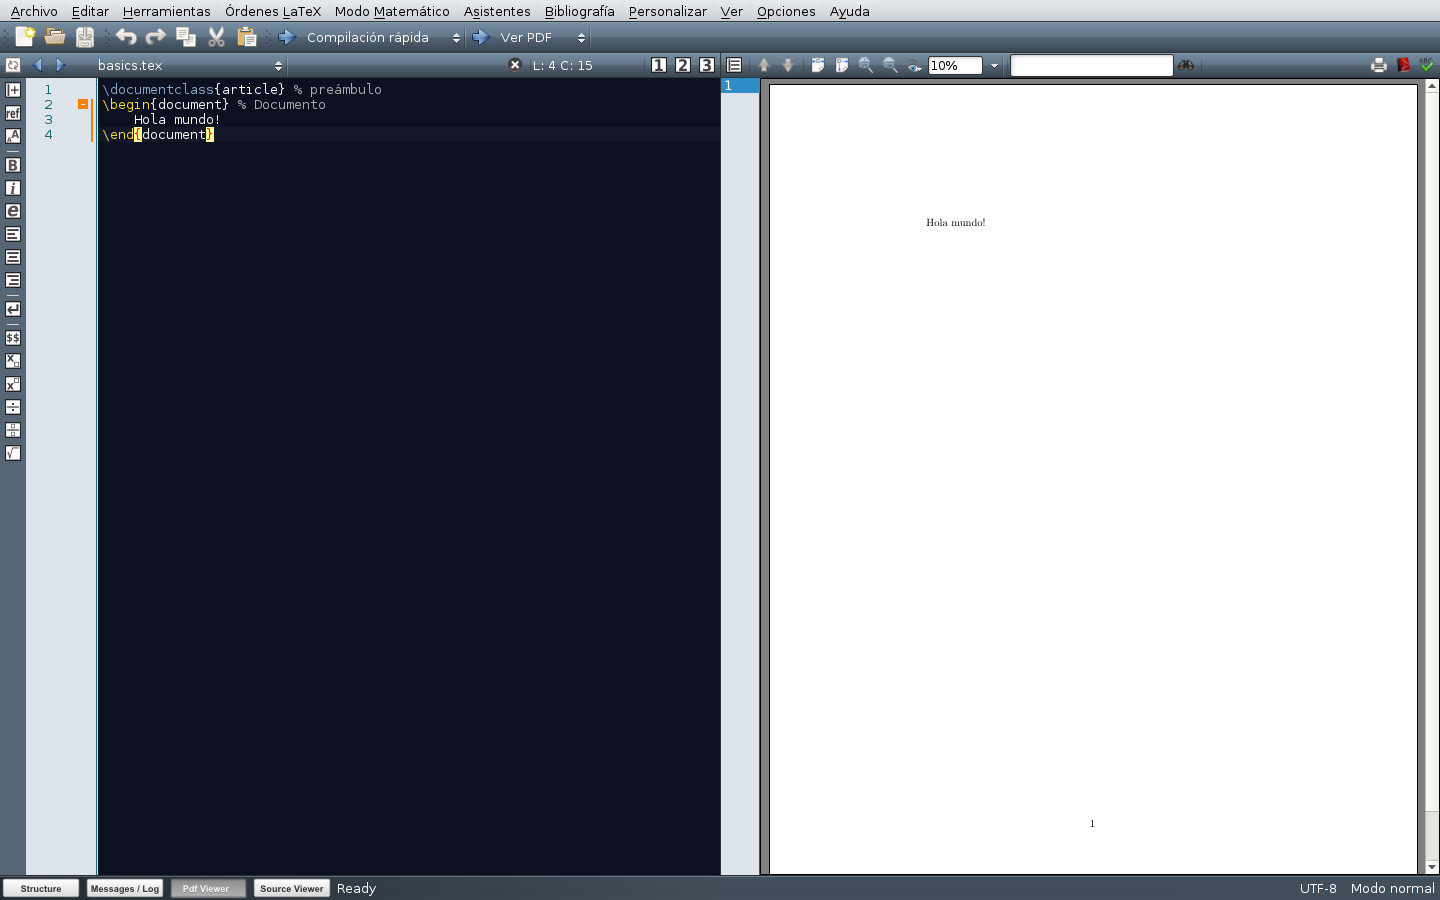
\includegraphics[scale = .25]{texmaker.jpg}
	\end{figure}
\end{frame}

\begin{frame}{Overleaf}
	\begin{figure}
		\centering
        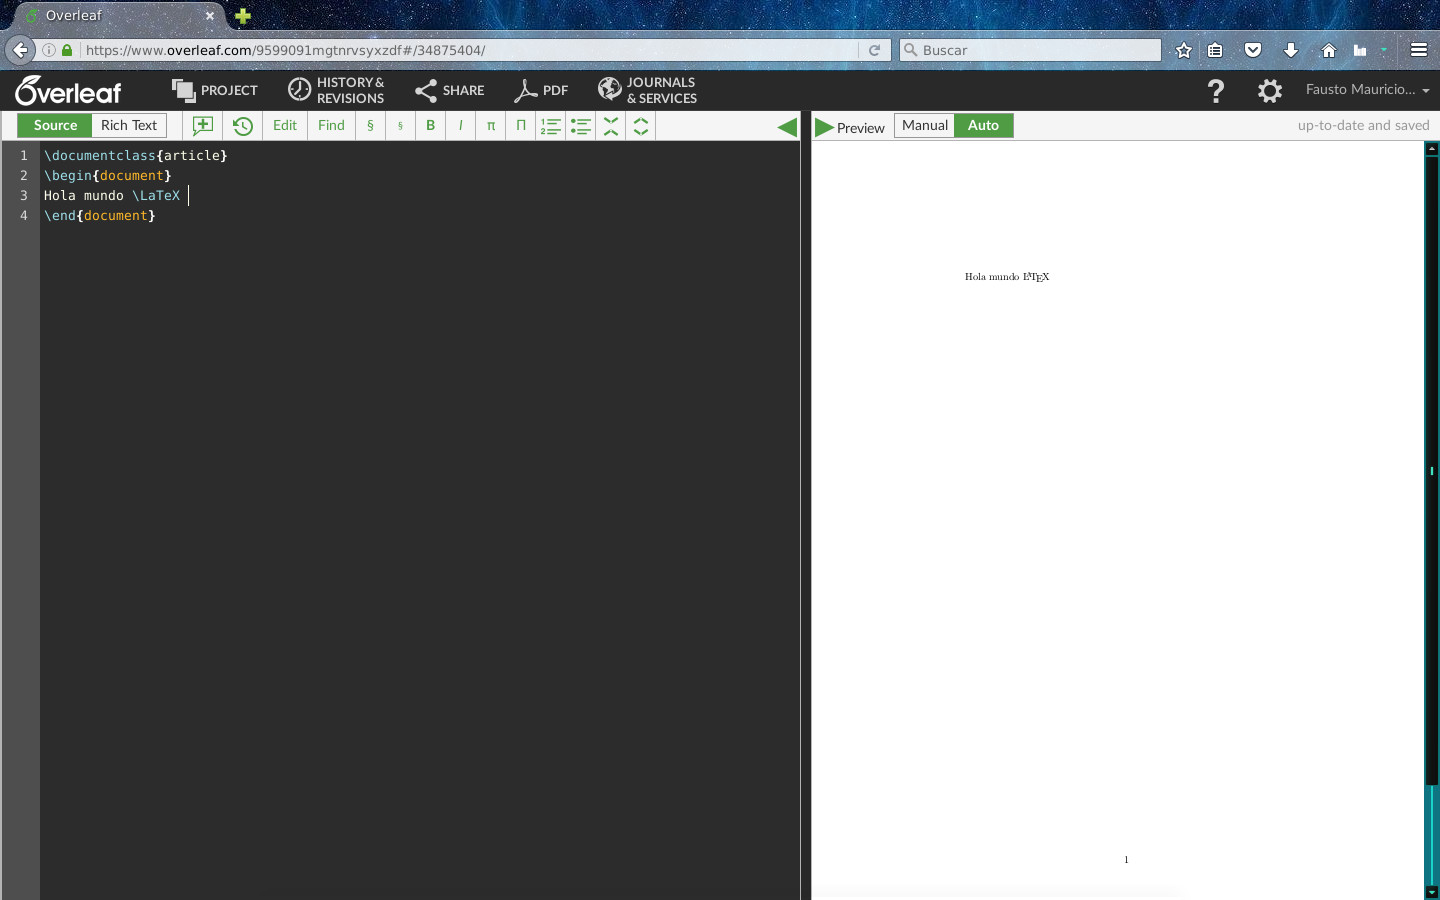
\includegraphics[scale = .25]{overleaf.jpg}
	\end{figure}
\end{frame}

\begin{frame}[c]{Símbolos y caracteres especiales}
	\begin{itemize}
		\item Uso de comillas: \\
        	Comillas simples \mintinline{latex}{`texto'} produce `texto' \\
            Comillas dobles \mintinline{latex}{``texto''} produce ``texto''.
        \item Algunos caracteres especiales \\
        	\begin{tabular}{cl}
        		\keystrokebftt{\%} & comentarios \\
                \keystrokebftt{\#} & argumentos de entrada \\
                \keystrokebftt{\&} & separador de tabulaciones \\
                \keystrokebftt{\$} & matemáticas en línea
        	\end{tabular}
        \item Para escribir alguno de estos caracteres especiales debe anteceder un \keystrokebftt{\bs}, e.g \mintinline{latex}{\$} produce \$.
	\end{itemize}
\end{frame}

\section{Escribiendo matemáticas}

\begin{frame}[fragile]{El signo \$}
	\begin{itemize}
		\item ¿Por qué es especial el signo \keystrokebftt{\$}? Porque se utiliza para escribir matemáticas dentro de una línea de texto.
\begin{exampletwouptiny}
% NO luce bien:
Sean a y b dos enteros positivos
diferentes, entonces c = a - b + 1.

% Luce bien:
Sean $a$ y $b$ dos enteros positivos
diferentes, entonces $c = a - b + 1$.
\end{exampletwouptiny}
\item Utilice siempre el signo \keystrokebftt{\$}, uno al inicio y otro al final de la expresión matemática.
\item \LaTeX{} ignora automáticamente los espacios.
\begin{exampletwouptiny}
Sea $y=mx+b$ entonces \ldots

Sea $y = m x + b$ entonces \ldots
\end{exampletwouptiny}
	\end{itemize}
\end{frame}

\begin{frame}[fragile]{Superíndices, subíndices y corchetes}
\small{
 \begin{table}[ht]
	 \begin{center}
	 \begin{tabular}{ l l }
	 	\hline
	 	\verb=|\,|= gives &  $|\,|$ \\
	 	\verb=|\;|= gives &  $|\;|$ \\
	 	\verb=|\quad|= gives &  $|\quad |$ \\
	 	\verb=|\qquad|= gives & $|\qquad|$ \\
	 	\verb=|\hspace{.5in}|= gives & $|\hspace{.5in}|$ \\
	 	\verb=|\hspace{6em}|= gives & $|\hspace{6em}|$ \\
   \hline
	 \end{tabular}
	 \end{center}
	 \end{table} 
	 }
	\begin{itemize}
		\item Utilice \keystrokebftt{\^} para superíndices y \keystrokebftt{\_} para subíndices.
        \item Utilice corchetes \keystrokebftt{\{} \keystrokebftt{\}} para escribir superíndices o subíndices grandes.
        \begin{exampletwouptiny}
$a_n = a_n-1 $ % error
$a_n = a_{n - 1}$ % correcto
$f(x) = e^ax + b - c$ % error
$f(x) = e^{ax + b} - c$ % correcto
        \end{exampletwouptiny}
        \item Existen comandos para las letras griegas y la notación común.
        \begin{exampletwouptiny}
$P(z)=\alpha+\lambda(z - \alpha)^n$
$\iint_Sdxdy = \iint_{H(S)}dxdy$
        \end{exampletwouptiny}
	\end{itemize}
\end{frame}

\begin{frame}{Documento clave}
\hspace{-.5cm}\footnotesize{\url{es.overleaf.com/latex/templates/a-quick-guide-to-latex/fghqpfgnxggz}}
\begin{figure}
    \centering
    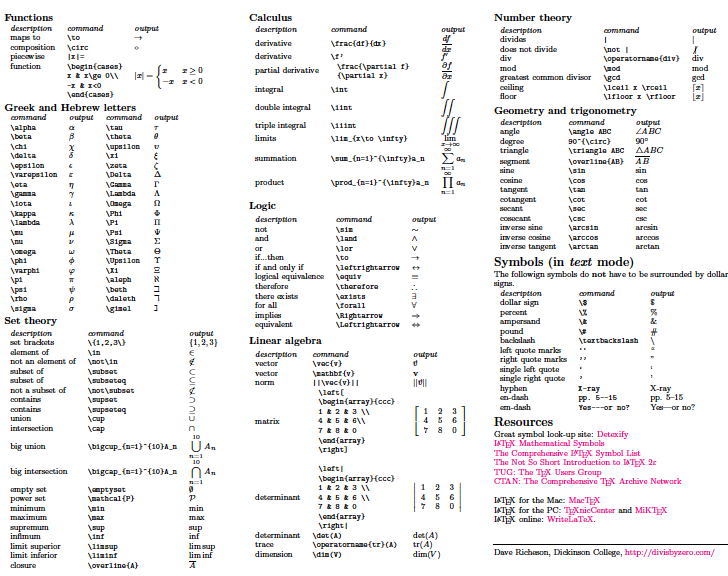
\includegraphics[scale = .35]{guide.png}
\end{figure}
\end{frame}
    

\section{Ambientes}

\begin{frame}[fragile]{Listas}
	\begin{itemize}
		\item Los comandos \cmdbs{begin} y \cmdbs{end} habilitan el uso de ambientes que son espacios ``especiales'' de un documento.
        \begin{exampletwouptiny}
\begin{itemize}
	\item Le\'on
	\item Tigre
	\item ...
\end{itemize}

\begin{enumerate}
	\item Criollo
    \item Angora
    \item ...
\end{enumerate}
        \end{exampletwouptiny}
        \item Fundamental los comandos \cmdbs{itemsep} (separación entre items) y \cmdbs{setlength}\{\cmdbs{itemindent}\}\{-2em\} (espacio horizontal items)
	\end{itemize}
\end{frame}

\begin{frame}[fragile]{\texttt{equation}}
	\begin{itemize}
		\item El ambiente \texttt{equation} presente de una forma elegante ecuaciones grandes.
    \begin{exampletwouptiny}
Las ra\'ices de la ecuaci\'on
cuadr\'atica est\'an dadas por
\begin{equation}
x = \frac{-b \pm \sqrt{b^2 - 4ac}}{2a}
\end{equation}
donde $a$, $b$ y $c$ son \ldots
    \end{exampletwouptiny}
    \item La presentación de ecuaciones varía entre el modo \texttt{inline} y el modo \texttt{display} (ambiente \texttt{equation})
    \begin{exampletwouptiny}
Escribir $\Omega = \sum_{k=1}^n \omega _k$
es diferente a escribir
\begin{equation}
\Omega = \sum_{k=1}^n \omega _k
\end{equation}
    \end{exampletwouptiny}
    
    \tiny{fíjese en la posición de los subíndices y superíndices de la suma.}
    \end{itemize}
\end{frame}

\section{Paquetes}

\begin{frame}[fragile]{paquete \texttt{amsmath}}
	\begin{itemize}
		\item Utilice \texttt{equation*} para ecuaciones no numeradas 
        \begin{exampletwouptiny}
\begin{equation*}
	\Omega = \sum_{k=1}^n \omega_k
\end{equation*}
	    \end{exampletwouptiny}
        \item \texttt{amsmath} define comandos para muchos operadores matemáticos
        \begin{exampletwouptiny}
\begin{equation*}
	\min_{x,y}{(1-x)^2 + 100(y-x^2)^2}
\end{equation*}
	    \end{exampletwouptiny}
        \item Puede definir operadores no incluidos en el paquete \linebreak con el comando \cmdbs{operatorname}.
        \begin{exampletwouptiny}
\begin{equation*}
	\beta_i =
    \frac{\operatorname{Cov}(R_i, R_m)}
    	{\operatorname{Var}(R_m)}
\end{equation*}
	    \end{exampletwouptiny}
	\end{itemize}
\end{frame}

\begin{frame}[fragile]{Alinear ecuaciones}
	\begin{itemize}
		\item Alinear una secuencia de ecuaciones con el ambiente \texttt{align*}
        \inputminted[frame = single]{latex}{align_environment.tex}
        \begin{align*}
       		\frac{r^2R'' + rR'}{R} + r^2\lambda^2 &= v^2 \\
        	r^2R'' + rR' + r^2\lambda^2R &= v^2R \\
        	r^2R'' + rR' + (\lambda^2r^2 - v^2)R &= 0.
        \end{align*}

        \item Utiliza \keystrokebftt{\&} para establecer el caracter de alineación y \keystrokebftt{\bs} \keystrokebftt{\bs} para iniciar una nueva línea.
	\end{itemize}
\end{frame}

\begin{frame}[c]{Crea tu comando}
\begin{figure}
    \centering
    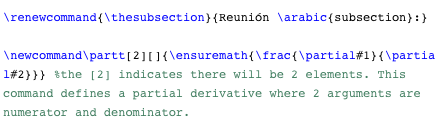
\includegraphics[scale=.65]{newcommand}
\end{figure}
	\begin{itemize}
	\item \partt[y]{x}
	\end{itemize}
\end{frame}

\begin{frame}[fragile]{Mendeley}
	Download: \url{https://chrome.google.com/webstore/detail/mendeley-web-importer/dagcmkpagjlhakfdhnbomgmjdpkdklff/related?hl=en-US} \\
	
	Reference sheet for natbib usage: \url{https://gking.harvard.edu/files/natnotes2.pdf}
	\newline
	\\
	\citet{Rossi2016a}
	\bibliographystyle{apalike}
	\bibliography{mendeley.bib}
\end{frame}

\begin{frame}[fragile]{Referencias Bibliográficas}
	\begin{itemize}
		\item El programa \bftt{Bibtex} produce la bibliografía en un documento \LaTeX{} a partir de una base de datos de referencias bibliográficas almacenada en un archivo \bftt{.bib}
        \item Puede cargarse cuantos archivos \bftt{.bib} sean necesarios mediante el comando \cmdbs{bibliography}
        \item Los nombres de los archivos \bftt{.bib} en el comando \cmdbs{bibliography} se separan con coma (,) y no necesitan llevar la extensión \bftt{.bib}
        \item El comando \cmdbs{bibliographystyle} define el estilo de presentación de las referencias bibliográficas.
        \item El comando \cmdbs{cite} cita una referencia bibliográfica en el documento
	\end{itemize}
\end{frame}

\section{Tablas}

\begin{frame}[fragile]{Tablas}
	\begin{itemize}\small{
		\item El paquete \cmdbs{tabular} permite crear arreglos de datos con o sin bordes (tablas)}
		\begin{exampletwouptiny}
\begin{tabular}{|c|c|}
    \hline
    celda 11 & celda 12 \\
    \hline
    celda 21 & celda 22 \\
    \hline
\end{tabular}
        \end{exampletwouptiny}
        \small{
		\item \LaTeX{} resuelve el problema de que cambien de lugar a medida uno agrega texto manipulando figuras y tablas como objetos flotantes.}
        \begin{minted}[frame = single, fontsize=\footnotesize]{latex}
            \begin{figure}[ubicación]
            ...
            \end{figure}
            \begin{table}[ubicación]
            ...
            \end{table}
        \end{minted}
        \item \small{La \emph{ubicación} puede ser \cmd{t} (top), \cmd{b} (botton) o \cmd{h} (here).}
	\end{itemize}
\end{frame}

\begin{frame}{Tablas}
        \small{
        \pgfplotstabletypeset[
    string type,
    columns/name/.style={column name=Name, column type={|l}},
    columns/surname/.style={column name=Surname, column type={|l}},
    columns/age/.style={column name=Age, column type={|c|}},
    every head row/.style={before row=\hline,after row=\hline},
    every last row/.style={after row=\hline},
    ]\mytable
\bigskip \\
\getcell{0}{name}{\mytable} \getcell{0}{surname}{\mytable} is \getcell{0}{age}{\mytable} 
years old. \getcell{1}{name}{\mytable} \getcell{1}{surname}{\mytable} is 
\getcell{1}{age}{\mytable} years old. But \getcell{2}{name}{\mytable} 
\getcell{2}{surname}{\mytable} is still older, he is \getcell{2}{age}{\mytable} years old.
        }
        \inputminted[fontsize=\scriptsize]{latex}{ref_table2_tab.tex}
\end{frame}

\begin{frame}[fragile]{Tablas}
        \inputminted[fontsize=\footnotesize]{latex}{ref_table2_pre.tex}
\end{frame}

\begin{frame}[fragile]{Tablas}
        \inputminted[fontsize=\scriptsize]{latex}{ref_table1_pre.tex}
        \\
        \begin{itemize}
        \setlength{\itemindent}{-1em}
        \small{
            \item Manual \cmdbs{pgfplotstable}: \url{http://pgfplots.sourceforge.net/pgfplotstable.pdf}
            \item Discusión en tex.stackexchange.com \url{tex.stackexchange.com/questions/86074/reference-table-value-in-text}
            }
        \end{itemize}
        \end{frame}

\section{Gráficos}
\begin{frame}[fragile]{Gráficos}
Links recomendados: \url{sites.google.com/site/kochiuyu/Tikz}
\url{texample.net/tikz/examples/area/economics/}
        \inputminted[fontsize=\scriptsize]{latex}{S-D.tex}
        \resizebox{.6\textwidth}{!}{
        \hspace{10cm}\begin{tikzpicture}[scale=0.6]
\draw[thick,<->] (0,10) node[above]{$P$}--(0,0)--(10,0) node[right]{$Q$};
\node [below left] at (0,0) {$0$};
\node [below] at (5,0) {$Q^*$};
\node [left] at (0,5) {$P^*$};
\draw(1,1)--(9,9) node[right]{$S$};
\draw(1,9)--(9,1) node[right]{$D$};
\draw[dashed](0,5)--(5,5)--(5,0);
\end{tikzpicture}
        }
\end{frame}

\begin{frame}[fragile]{Gráficos}
        \inputminted[fontsize=\scriptsize]{latex}{area.tex}
        \resizebox{.8\textwidth}{!}{
        \hspace{10cm}\begin{tikzpicture}
\draw[thick,<->] (0,7) node[above]{$p$}--(0,0)--(8,0) node[right]{$q$};
\draw (0,6)--(6,0) node[above right]{D};
\draw (0,3) --(5,3) node[right]{$c_0$};
\draw(0,2) --(5,2) node[right]{$c_1$};
\draw[dashed] (0,4) node[left]{$p_1$}--(2,4)--(2,0) node[below]{$q_1$};
\draw[dashed] (0,3) node[left]{$p_0$}--(3,3)--(3,0) node[below]{$q_0$};
\path[pattern=horizontal lines,pattern color=red] (2,4)--(2,3)--(3,3);
\path[pattern=vertical lines,pattern color=blue] (0,3)--(2,3)--(2,2)--(0,2);
\end{tikzpicture}
        }
\end{frame}

 \begin{frame}{}
  \vspace{-.2cm}
        \inputminted[fontsize=\tiny]{latex}{intersection.tex}
        \vspace{-1.1cm}
        \begin{flushright}
      \resizebox{.3\textwidth}{!}{
        \begin{tikzpicture}[
    scale=5,
    axis/.style={very thick, ->, >=stealth'},
    important line/.style={thick},
    dashed line/.style={dashed, thin},
    pile/.style={thick, ->, >=stealth', shorten <=2pt, shorten>=2pt},
    every node/.style={color=black}]
    % axis
    \draw[axis] (-0.1,0)  -- (1.1,0) node(xline)[right] {$G\uparrow/T\downarrow$};
    \draw[axis] (0,-0.1) -- (0,1.1) node(yline)[above] {$E$};
    % Lines
    \draw[important line] (.15,.15) coordinate (A) -- (.85,.85) coordinate (B) 
    node[right, text width=5em] {$Y^O$};
    \draw[important line] (.15,.85) coordinate (C) -- (.85,.15)
        coordinate (D) node[right, text width=5em] {$\mathit{NX}=x$};
    % Intersection of lines
    \fill[red] (intersection cs: first line={(A) -- (B)},
       second line={(C) -- (D)}) coordinate (E) circle (.4pt) node[above,] {$A$};
    % The E point is placed more or less randomly
    \fill[red]  (E) +(-.075cm,-.2cm) coordinate (out) circle (.4pt) node[below left] {$B$};
    % Line connecting out and ext balances
    \draw [pile] (out) -- (intersection of A--B and out--[shift={(0:1pt)}]out) coordinate (extbal);
    \fill[red] (extbal) circle (.4pt) node[above] {$C$};
    % line connecting  out and int balances
    \draw [pile] (out) -- (intersection of C--D and out--[shift={(0:1pt)}]out) coordinate (intbal);
    \fill[red] (intbal) circle (.4pt) node[above] {$D$};
    % line between out og all balanced out :)
    \draw[pile] (out) -- (E);
\end{tikzpicture}
        }
        \end{flushright}
  \end{frame}
  
  \begin{frame}[fragile,c]{Gráficos}
        \resizebox{.8\textwidth}{!}{
        \hspace{10cm}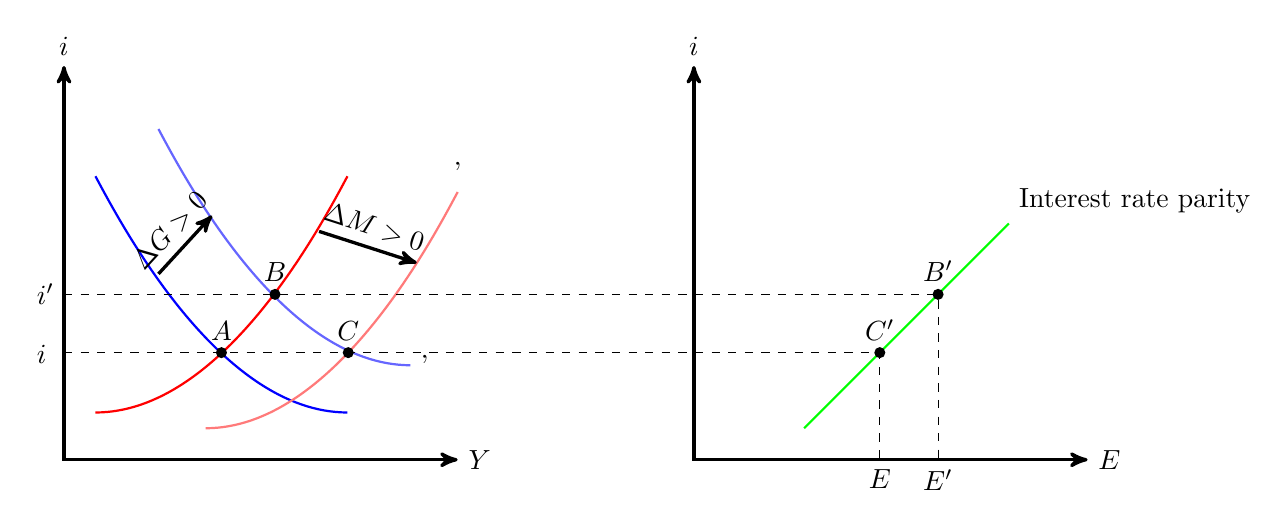
\begin{tikzpicture}[
        scale=2,
        IS/.style={blue, thick},
        LM/.style={red, thick},
        axis/.style={very thick, ->, >=stealth', line join=miter},
        important line/.style={thick}, dashed line/.style={dashed, thin},
        every node/.style={color=black},
        dot/.style={circle,fill=black,minimum size=4pt,inner sep=0pt,
            outer sep=-1pt},
    ]
    % axis
    \draw[axis,<->] (2.5,0) node(xline)[right] {$Y$} -|
                    (0,2.5) node(yline)[above] {$i$};
    % IS-LM diagram
    \draw[LM] (0.2,0.3) coordinate (LM_1) parabola (1.8,1.8)
        coordinate (LM_2) node[above] {\LM};
    \draw[IS] (0.2,1.8) coordinate (IS_1) parabola[bend at end]
         (1.8,.3) coordinate (IS_2) node[right] {\IS};
    %Intersection is calculated "manually" since Tikz does not offer
    %intersection calculation for parabolas
    \node[dot,label=above:$A$] at (1,.68) (int1) {};
    %shifted IS-LM diagram
    \draw[xshift=.7cm, LM, red!52] (0.2,0.2) parabola (1.8,1.7)
        node[above] {\LM'};
    \draw[xshift=.4cm, yshift=.3cm, IS, blue!60] (0.2,1.8)
        parabola[bend at end] (1.8,.3)
        node[right] {\IS'};
    %Intersection of shifted IS-LM
    \path[xshift=.36cm, yshift=.35cm] (.98,.7)
        node[dot,label=above:{$B$}] (int2) {};
    \path[xshift=.805cm] (1,.68) node[dot,label=above:$C$] (int3) {};
    %arrows between intersections
    \draw[->, very thick, black, >=stealth']
        ($(int1)+1/2*(-.80,1)$) -- ($(int2)+1/2*(-.8,1)$)
        node[sloped, above, midway] {$\mathsmaller{\Delta G > 0}$};
    \draw[->, very thick, black, >=stealth']
        ($(int2)+2*(.14,.2)$) -- ($(int2)!.2cm!270:(int2)+(.9,0)$)
        node[sloped,above, midway] {$\mathsmaller{\Delta M>0}$};
        
    \begin{scope}[xshift=4cm]
        %E-diagram
        \draw[axis,<->] (0,2.5) node(eyline)[above] {$i$} |-
                        (2.5,0) node(exline)[right] {$E$};

        \draw[important line, green, xshift=.5cm]
            (.2,.2) coordinate (es) -- (1.5,1.5) coordinate (ee)
            node [above right] {Interest rate parity};
    \end{scope}
    %Lines connecting IS LM coordinates and E coordinates
    \draw[dashed] 
        let
            % Store the intersection point in \p1 for later retrieval. 
            % A convenient feature of the let operation is that we can
            % access the x and y component of the coordinate directly 
            % using the \x1 and \y1 syntax. 
            \p1=(intersection of int2--[xshift=1]int2 and es--ee)
        in
            (0,\y1) node[left]{$i'$} -|  (\x1,0)
            node[pos=0.5,dot,label=above:$B'$] {} node[below] {$E'$};

    \draw[dashed line] let
        \p1=(intersection of int3--[xshift=1]int3 and es--ee)
            in
        (0,\y1) node[left]{$i\phantom{'}$} -| (\x1,0)
        node[dot,label=above:$C'$,pos=0.5] {} node[below] {$E$};

\end{tikzpicture}

        }
        \resizebox{.8\textwidth}{!}{
        \hspace{7cm}  \begin{tikzpicture}[scale=1]
    % Axis
    \coordinate (y) at (0,5);
    \coordinate (x) at (5,0);
    \draw[<->] (y) node[above] {$r$} -- (0,0) --  (x) node[right]
    {$\mathit{EV}$};
    % A grid can be useful when defining coordinates
    % \draw[step=1mm, gray, thin] (0,0) grid (5,5); 
    % \draw[step=5mm, black] (0,0) grid (5,5); 

    % Let us define some coordinates
    \path
    coordinate (start) at (0,4)
    coordinate (c1) at +(5,3)
    coordinate (c2) at +(5,1.75)
    coordinate (slut) at (2.7,.5)
    coordinate (top) at (4.2,2);

    \draw[important line] (start) .. controls (c1) and (c2) .. (slut);
    % Help coordinates for drawing the curve
    % \filldraw [black] 
    % (start) circle (2pt)
    % (c1) circle (2pt)
    % (c2) circle (2pt)
    % (slut) circle (2pt)
    \filldraw [black] 
     (top) circle (2pt) node[above right, black] {$Q$};

     % We start the second graph
     \begin{scope}[xshift=6cm]
       % Axis
      \coordinate (y2) at (0,5);
      \coordinate (x2) at (5,0);
      \draw[axis] (y2) node[above] {$r$} -- (0,0) --  (x2) node[right] {$L$};
      % Define some coodinates
     \path
     let
     \p1=(top)
     in
     coordinate (sstart) at (1,.5) 
     coordinate (sslut) at (4, 4.5)
     coordinate (dstart) at (4,.5)
     coordinate (dslut) at (1,4.5)
% Intersection 1
     coordinate (int) at  (intersection cs:
       first line={(sstart)--(sslut)},
       second line={(dstart)--(dslut)})
% Intersection 2
    coordinate (int2) at  (intersection cs:
       first line={(top)--($(10,\y1)$)},
       second line={(dstart)--(dslut)})
% Intersection 3
    coordinate (int3) at  (intersection cs:
       first line={(top)--($(10,\y1)$)},
       second line={(sstart)--(sslut)});
% Draw the lines
     \draw[important line] (sstart) -- (sslut) node[above right] {$S$}
       (dstart) -- (dslut)  node[above left] {$D$};
     \draw[connection] let \p1=(int2), \p2=(int3) in 
     (int2)--(\x1,0) node[below] {$\mathit{L_D}$}
     (int3)--(\x2,0) node[below] {$\mathit{L_S}$};
      \end{scope}
%Finally, connect the two graphs
     \draw[connection] let \p1=(top), \p2=(x2) in (0,\y1) node[left]
     {$r^*$} -- (\x2, \y1);
    \end{tikzpicture}
        }
\end{frame}
  

\section{Templates} 
     \begin{frame}[c]{Templates}
     \begin{itemize}
         \item Beamer: \url{www.overleaf.com/gallery/tagged/presentation}
         \item La que yo uso Beamer: \url{www.overleaf.com/read/fqybkcdgrdnr}
         \item Para papers que yo armé: \url{www.overleaf.com/read/hrvmddfhxjzz}
     \end{itemize}

  \end{frame}

\end{document}